\documentclass [a4paper, 11pt]{article}

\usepackage{amsmath,amssymb}
\usepackage{epsfig}
\usepackage{graphicx}
\usepackage{times}
\usepackage{float}
\usepackage[usenames,dvipsnames]{color}
\usepackage{hyperref}
\usepackage{scrlayer-scrpage}
\usepackage{subfigure}
\usepackage{cleveref}
\usepackage{bm}
\pagestyle{scrheadings}
\clearpairofpagestyles

\textwidth 16 cm
\textheight 23 cm
\setlength{\oddsidemargin}{0.1 cm}
\setlength{\topmargin}{1 cm}
\setlength{\headheight}{0cm}
\setlength{\headsep}{0cm}
\setlength{\footskip}{0.75cm}
\setlength{\parindent}{0cm}
\setlength{\oddsidemargin}{0.1 cm}
\setlength{\itemsep}{10pt}
\bibliographystyle{gcs}
\cfoot{\pagemark}
\ofoot{\tiny V1.9-2022JUL06}

\newcommand{\Pvec}{\mathbf{P}}

\begin{document}

\LARGE
\begin{center}
	\bf Project Report\\
\end{center}

\large
\bigskip
\bigskip
\bigskip

\textbf{Type of report}\\
\phantom{MM}\textit{“Status Report”}

\bigskip
\textbf{Period}\\
\phantom{MM}\textit{10.2023-9.2024}

\bigskip
\textbf{Project title}\\
\phantom{MM}\textit{Inclusive semileptonic decay rates from lattice QCD}

\bigskip
\textbf{HPC system(s) and corresponding centres(s)}\\
\phantom{MM} \textit{JUWELS Booster, JSC}

\bigskip
\textbf{Project ID}\\
\phantom{MM} \textit{ISDLQCD}

\textbf{Principal investigator}\\
\phantom{MM} \textit{C. Urbach, Helmholtz-Institut für Strahlen- und Kernphysik (Theorie) and
	Bethe Center for Theoretical Physics, University of Bonn, 53115 Bonn, Germany}

\bigskip
\textbf{Project contributor(s)}\\

\phantom{MM} \textit{
	A.~Evangelista$^a$,
	R.~Frezzotti$^a$,
	G.~Gagliardi$^b$,
	M.~Garofalo$^c$,
	C.~Groß$^c$,
	B.~Kostrzewa$^d$,
	V.~Lubicz$^e$,
	M.~Panero$^f$,
	F.~Sanfilippo$^b$,
	S.~Simula$^b$,
	A~Smecca$^g$,
	N.~Tantalo$^a$
}\\


\textit{$^a$ Dipartimento di Fisica and INFN, Universit\`a di Roma ``Tor Vergata", Via della Ricerca Scientifica 1, I-00133 Roma, Italy}\\
\textit{$^b$ Instituto Nazionale di Fisica Nucleare, Sezione di Roma Tre, Via della Vasca Navale 84, I-00146 Rome, Italy }\\
\textit{$^c$ Helmholtz-Institut f{\"u}r Strahlen- und Kernphysik (Theorie) and Bethe Center for Theoretical Physics, Universit{\"a}t Bonn}\\
\textit{$^d$ High Performance Computing and Analytics Lab, University of Bonn, 53115 Bonn, Germany} \\
\textit{$^e$ Dipartimento di Matematica e Fisica, Universit\`a Roma Tre and INFN, Sezione di Roma Tre, Via della Vasca Navale 84, I-00146 Rome, Italy} \\
\textit{$^f$ Dipartimento di Fisica, Università di Torino \& INFN, Sezione di Torino, Via Pietro Giuria 1, I-10125 Turin, Italy}\\
\textit{$^g$ Department of Physics, Faculty of Science and Engineering, Swansea University (Singleton Park Campus) Singleton Park, SA2 8PP Swansea, Wales, United Kingdom}

\newpage

\vfill
\tableofcontents
\vfill

\newpage

\section{Abstract}\label{sec:abstract}
\rule{\textwidth}{0.4pt}
%\textit{Give a short introduction to the project and stress the highlights.}\\


Flavour physics is an important and active research topic, it has high potential
for the discovery of a statistically significant discrepancy between the SM and
experiment.
Even if the mass scales of new
particles beyond the SM turned out to be very high, quantum effects of
the associated fields could leave detectable imprints on the physics
of heavy quarks.
This indicates the need for precise theoretical computations from
first principles of observables related to semi-leptonic decays of
heavy mesons and elements of the CKM matrix. 

With the computer time granted to us in the current granting period we
were able to perform a fully non-perturbative computation of the inclusive semileptonic
decay rate of the $D_s$ meson.
A first principles computation of this decay rate is of high
phenomenological relevance, since a comparison with experimental data
allows for stringent Standard Model tests in the sector of Flavour physics.
Additionally, our work sets the stage to a future
project involving the $B$ meson(s), which will allows us to
investigate current flavour anomalies.



\section{Scientific work accomplished and results obtained}\label{sec:results}
\rule{\textwidth}{0.4pt}

In the current accounting period we were so far able to run the
proposed jobs according to our schedule. Since the granted computing
time was less than what we proposed, we had changed our plan
accordingly.
However, by reducing our target the statistics from 400 gauge
configurations per ensemble to 300, and by reducing the
number of stochastic sources by a factor two,
% and using other time 
% available to us in other machines (LEONARDO booster at CINECA)
we could
generate enough data to perform our calculation, while slightly
sacrificing the statistical precision. 
% However, due to extra time available to us due to JUWELS
% being idle otherwise, we could nevertheless generate according to plan.

The gauge ensembles we use to generate data are compiled in Table~\ref{tab:ensembles}.
With respect to our proposal, we replace the ensemble cAp211.077.64
with the cB211.072.48, the latter being computationally
cheaper. However, with this change we have three ensembles with all
parameteres but the volume equal, which provides us with very valuable
insights into finite volume effects.

With this improved control over finite volumen effects, we could then
replace also ensemble cC211.06.112 with cE211.044.112. Both 
ensembles come with similar computational costs, but the cE211.044.112
is at a finer lattice spacing allowing us to perform a better
controlled continuum limit, while finite volume effects are controlled
by the three cB ensembles.

Despite ongoing simulation efforts, our preliminary results
look very promising and a paper is in preparation.  
Moreover, the results obtained with the resources granted to this
project have been presented in different talks at the 41st
International Symposium on Lattice Field Theory, which took place from
September 28 to August 3 of this year in Liverpool, UK.


\begin{table}[h]
  \centering % center the table
  \begin{tabular}{lccccr} % alignment of each column data
    \hline
    name          & $L$ [fm]      & $a$
    [fm]          & $M_\pi$ [MeV] & $M_\pi L$                         \\
    \hline
		% cAp211.077.64 & 5.76 & $\sim$0.09 & $\approx$ 135 & 3.95  \\
    \hline
    cB211.072.48  & 3.84          & $\sim$0.08 & $\approx$ 135 & 2.63 \\
    cB211.072.64  & 5.12          & $\sim$0.08 & $\approx$ 135 & 3.51 \\
    cB211.072.96  & 7.68          & $\sim$0.08 & $\approx$ 135 & 5.27 \\
    \hline
    cC211.06.80   & 5.44          & $\sim$0.07 & $\approx$ 135 & 3.72 \\
    % cC211.06.112  & 7.62          & $\sim$0.07 & $\approx$ 135 & 5.21 \\
    \hline
    cD211.054.96  & 5.76          & $\sim$0.06 & $\approx$ 135 & 3.94 \\
    \hline
    cE211.044.112 & 5.48          & $\sim$0.05 & $\approx$ 135 & 3.75 \\
    \hline
  \end{tabular}
  \caption{ETMC's $N_f=2+1+1$ gauge ensembles relevant for this
    proposal. The time extent is always set to $T=2L$.}
  \label{tab:ensembles}
\end{table}

\subsection{Sub-project 1: Total inclusive decay rate $D_s \to X\ell\nu$}

The total inclusive decay rate for the
process $D_s \to X\ell\nu$ can be written as
\begin{equation}
	\Gamma = G^2_F\left\{ |V_{cd} |^2 \Gamma_{cd} + |V_{cs} |^2 \Gamma_{cs} + |V_{us} |^2 \Gamma_{su}
	\right\}\,,
\end{equation}
where the different contributions on the right hand side correspond at the quark level to the weak
transitions $c \to d$, $c \to s$, and $s \to u$, respectively.
The contribution $su$ is suppressed by the integration over the phase
space thus expected to be negligible. So far, we have computed only
the contribution coming from the channels $cd$ and $cs$ and the
computaiton of the $su$ channel is still ongoing.
Each term can be computed
\begin{equation}
	\frac{48 \pi^4}{m_{B_{(s)}}^5}\frac{d\Gamma_{fg}}{d \bm{ q^2} }
	=\lim_{\sigma\to 0}\sum_{l=0}^2 |\bm{q}|^{3-l}\int_0^{\infty}d q_0 (q^{max}_0-q_0)^l\Theta_\sigma(q_0^{max},q_0) Z^l\,.
	\label{eq:gamma}
\end{equation}
The above integral can be computed with the HLT method \cite{Hansen:2019idp} reconstructing the
convolution of the spectral
density $Z$  with the kernel $\Theta_\sigma$.
In the HLT method, the kernel $\Theta_\sigma$ gets replaced by an
approximate kernel $\sum_{\tau=1}^Ng_\tau e^{-\omega_0\tau}$, where
$N$ is the number of time slices used in the spectral recontruction,
and $g$ are parameters to be determined minimizing the function 
\begin{equation}
  W[\lambda, g]=(1-\lambda)\frac{A[g]}{A[0]}+\lambda B[g]\,.
  \label{eq:W_HLT}
\end{equation}
The systematic error in approximating the kernel is given by
$A[g]=\int_{E_0}^\infty d \omega_0( \sum_{\tau=1}^N g_\tau e^{-\omega_0\tau}- \Theta_\sigma )^2$
and the statistical error by $B[g]=\bm{g}^T
\mbox{COV}[C(t)]\bm{g}$ with correlator $C(t)$. $\lambda$ represents a
trade-off of parameter to balance systematic versus statistical
error. The effect of $\lambda$ on the decay rate is shown in
Figure~\ref{fig:stability}, where we see that there is a window in
$\lambda$ where the result is stable. 

\begin{figure}
  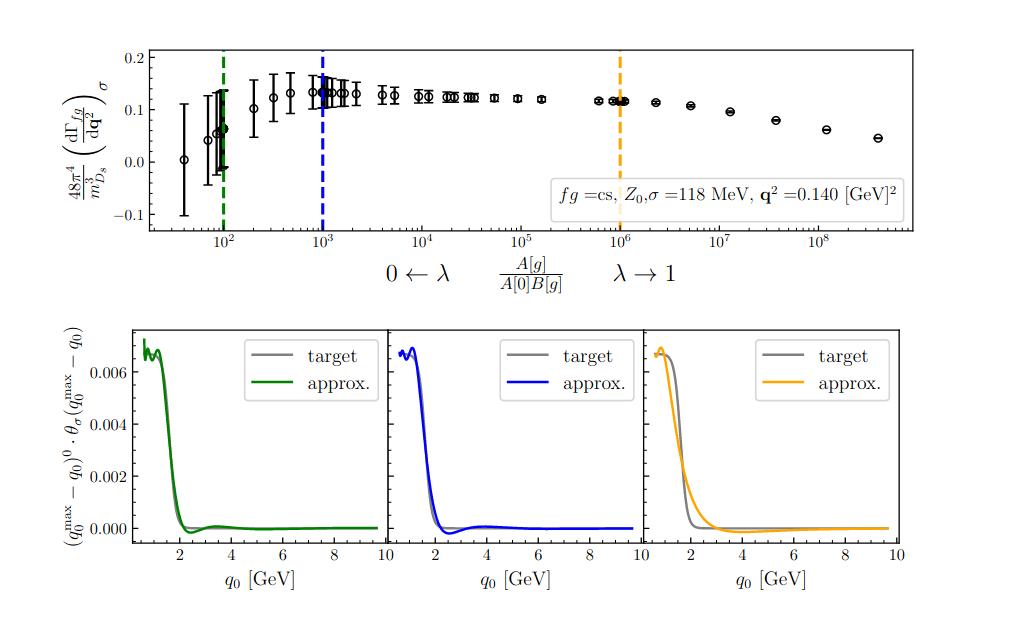
\includegraphics[scale=0.5]{figures/Screenshot from 2024-07-27 18-12-04.png}
  \caption{Values of the decay width obtained from different values of $\lambda$, the trade-off
    parameter of Eq.~\ref{eq:W_HLT} in the top panel. In the panels below we show the kernel $\Theta_\sigma$ against the kernel reconstructed from the HLT method at the values of  $\lambda$ corresponding to
    marked by vertical dashed lines in the panel above.
  }
  \label{fig:stability}
\end{figure}

% with the data produced we also observed that 
% our calculation the  extrapolation $\sigma \to 0$ can been done 
Another central point in our project is the $\sigma \to 0$
extrapolation. Only in this limit the physical decay rate is obtained.
As visible in Figure~\ref{fig:sigma_extrapolation}, the
$\sigma \to 0$ extrapolation is smooth and can be described by 
a polynomial function in $\sigma$. Therefore, we expect to be able to
control the corresponding uncertainties.

\begin{figure}
  \centering
  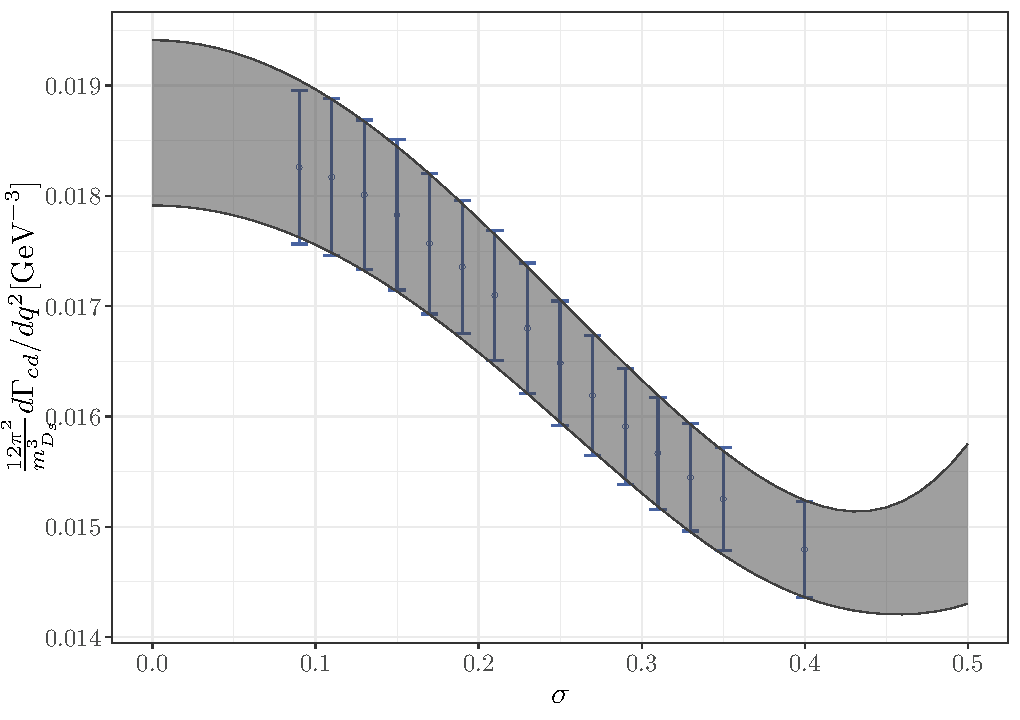
\includegraphics[scale=0.5]{figures/sigma_extrapolation.pdf}
  \caption{ $\sigma \to 0 $ extrapolation for the decay width in the
    $cu$ flavour channel for $q^2\approx 0.04$. 
  }
  \label{fig:sigma_extrapolation}
\end{figure}

For the total inclusive decay rate $D_s \to X\ell\nu$, the usage of three volumes
at the same lattice spacing (cB211.072.48, cB211.072.64 and cB211.072.96)
gives us control over the finite volume effects. As we can see in Fig.~\ref{fig:dGamma_FSE_B},
there is no sign of finite volume effects with the present statistical
uncertainties, which is the main reason for the aforementioned
replacement of ensemble cC211.06.112 with the finer lattice spacing
ensemble cE211.044.112.
An example for the continuum limit of the differential decay rate at
specific squared momentum $q^2=0.7\,\mathrm{GeV}^2$ is shown in
Figure~\ref{fig:dGamma_continuum}. We find that the 
$\mathbf{O}(a^2)$ lattice artefacts are negligible given our current
statistical uncertainties. The gray band represents a preliminary
constant continuum extrapolation. However, one also observes from the
figure that the ensemble cC211.06.112, responsible for the second data point
from the right, likely requires more statistics in the future.

\begin{figure}
  \begin{center}
    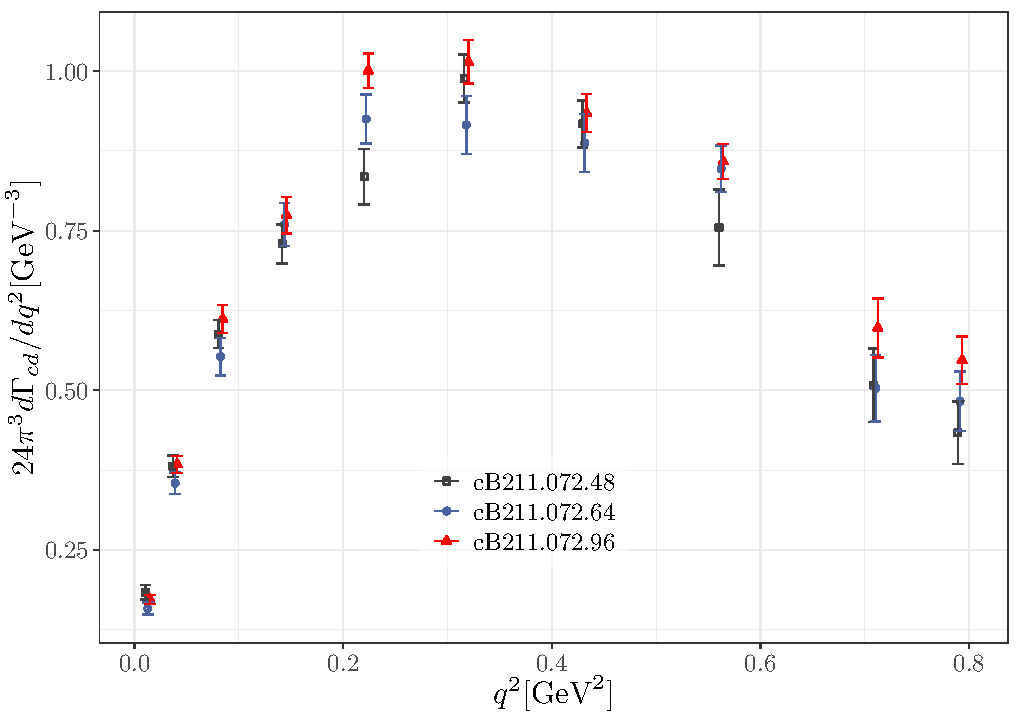
\includegraphics[scale=0.7]{figures/dGamma_FSE_B.pdf}
    \caption{Values of $d\Gamma_{cd}/dq^2$ for the $cd$ flavour
      channel obtained at three different volumes, and otherwise equal
      parameters of the three cB211.072 ensembles.}
    \label{fig:dGamma_FSE_B}
  \end{center}
\end{figure}

\begin{figure}
  \begin{center}
    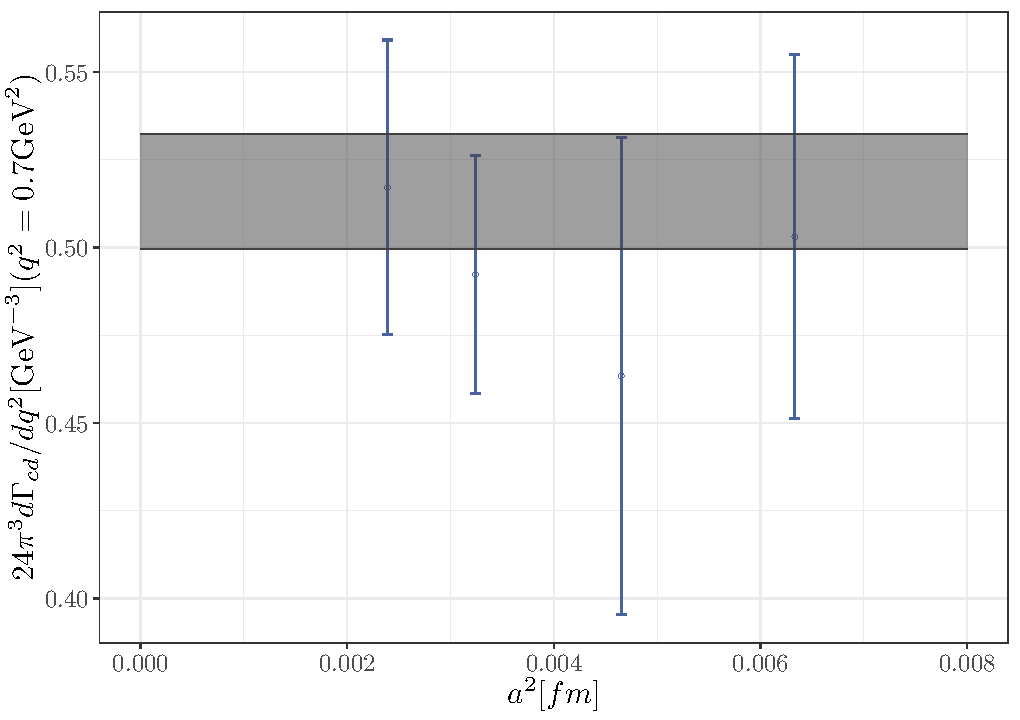
\includegraphics[scale=0.7]{figures/dGamma_continuum_th9.pdf}
    \caption{$d\Gamma_{cd}/dq^2$ at $q^2=0.7\,\mathrm{GeV}^2$ for the
      $cd$ flavour channel. The gray band represents a constant
      continuum extrapolation.}
    \label{fig:dGamma_continuum}
  \end{center}
\end{figure}

Finally, we show in Figure~\ref{fig:gamma_cs_cd} a comparison of the
contributions from the two different flavour channels, with the $cs$
channel in the left and the $cd$ channel in the right panel.
We show the three $Z_i$ separately for $i=0,1,2$, but normalise with
the appropriate CKM matrix element, i.e. $V_{cs}^2$ in the left and
$V_{cd}^2$ in the right panel, leading to a significant suppression of
the $cd$ contribution compared to the $cs$ contribution.


\begin{figure}
  \begin{center}
    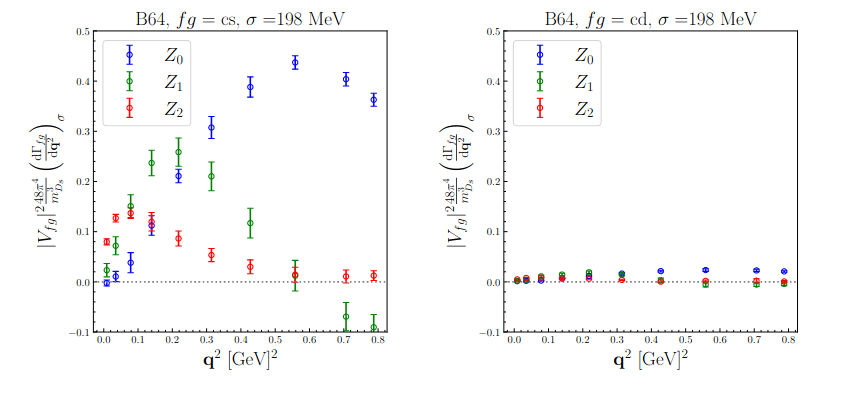
\includegraphics[scale=0.5]{figures/Screenshot from 2024-07-27 19-31-31.png}
    \caption{We show the decay rate mutpliplied with the appropriate
      squared CKM matrix element as a function of $q^2$, in the left
      panel for the $cs$ flavour channel, in the right panel for $cd$,
      for the three $Z_i$ separately.}
    \label{fig:gamma_cs_cd}
  \end{center}
\end{figure}

In the remaining time of the project we will focus on computing the
$su$ flavour channel and verifying the
theoretical expectation that it is suppressed compared to the other
channels. Further, we will perform an extra run to check the effect of a 
possible mistuning of the quark mass of the charm and strange as well
as finalizing the analysis and prepare a publication. 


\subsection{Sub-project 2: decay constant $f_D$ and $f_{D_s}$}

The decay constant of a pseudo-scalar (PS) meson with flavours $f$ and
$f'$ can be extracted from the equation
\begin{equation}
  f_\mathrm{PS}=(\mu_f+\mu_{f'})\frac{\langle 0| P_{ff'}|
    \mathrm{PS}\rangle}{M_\mathrm{PS}^{ff'}\sinh(M_\mathrm{PS}^{ff'})}\,
\end{equation}
where the matrix element in the nominator can be extracted from the
correlation function $\langle O_\mathrm{PS}(t)O_\mathrm{PS}(t)^\dagger
\rangle$ at large Euclidean time separations. The PS-meson is composed of
valence quark flavours with bare masses $\mu_f$ and $\mu_{f'}$,
its mass is denoted by $M_\mathrm{PS}^{ff'}$ and the corresponding interpolating
operator is $O_\mathrm{PS}=\bar f \gamma_5 f' $. We plan to compute the
decay constant for the $D_s$ and $D$ meson, thus $f=c$ and $f'=s,d$.

We produced all the data necessary to extract the decay constant for
all the ensemble listed in Table~\ref{tab:ensembles}, and the analysis
is ongoing.



\section{Realization of the project}
\rule{\textwidth}{0.4pt}\\


We have produced data running from 2 to 56 nodes of Juwels Booster
depending on the ensemble size. Data for both sub-projects are
produced in the same runs.
We managed to further optimise the memory footprint of our code
(nissa~\footnote{\url{https://github.com/sunpho84/nissa}}). This made
it possible to reduce the number of nodes used in runs for the
cB211.072.64 ensemble from 8 to 4, and for the cC211.06.80 ensemble
from 20 to 10. This reduction in the number of nodes increased the
efficiency of our runs by a factor of about 1.2.

\section{Publications with the appropriate acknowledgement}
\rule{\textwidth}{0.4pt}

We are preparing a publication with our result of the inclusive decay rate $D_s\to X\ell\nu$ and 
preliminary result were presented at the Lattice conference 2024 
\cite{talklatt2024_ale,talklatt2024_chr}.

\begin{thebibliography}{99}



\end{thebibliography}


\section{Theses completed within the project}
\rule{\textwidth}{0.4pt}

There are no theses to report.

\section{Additional references}
\rule{\textwidth}{0.4pt}

\bibliography{biblio}

\section{Material suitable for the general public}
\rule{\textwidth}{0.4pt}

Currently, we do not yet have such material available.


\end{document}
